%!TEX root = ../template.tex
%%%%%%%%%%%%%%%%%%%%%%%%%%%%%%%%%%%%%%%%%%%%%%%%%%%%%%%%%%%%%%%%%%%%
%% chapter2.tex
%% NOVA thesis document file
%%
%% Chapter with the template manual
%%%%%%%%%%%%%%%%%%%%%%%%%%%%%%%%%%%%%%%%%%%%%%%%%%%%%%%%%%%%%%%%%%%%

\chapter{Characterization of data sets}
\label{cha:general_characterization}

\hspace{10px} One of the main challenges of the present time is to correctly discover and identify the alterations in the genome that lead to the appearance of cancer. Through these molecular anomalies, researchers are able to unravel how cancer develops, as well as help to perfect treatment methods and correct diagnosis of the type of cancer. In support, the GDC assists researchers by providing access to regulated clinical and genomic data from different cancer studies to facilitate in exploratory analysis to identify changes in cancer cells that may play an important role in cancer development. Through the \glsxtrshort{GDC} knowledge base, it is possible to leverage the data contained in the GDC to help identify high and low frequency cancer factors such as mutations (through the data is generated the \glsxtrshort{VCF} and \glsxtrshort{MAF} files that identify point mutations, missense mutations, nonsense mutations, insertions and deletions), Copy Number Variations or CNV (data help to identify amplified and attenuated gene expression due to chromosomal duplications, loss, insertions and deletions), expression quantification (access to mRNA and miRNA sequence data and quantifies gene and miRNA expression using regulated software pipelines) and post-transcriptional modifications (access to mRNA sequence data to assist in identifying post-transcriptional splice modifications that are manifested as splice junction and isoform variant). For this work, the main focus will be only on files of type MAF. Unlike CNVs, which include both duplications and deletions along with inversions and translocations that change the structure of the genome, being classified as forms of structural variation in the genome or \gls{SV}, these variations can affect 2 or more contiguous genes, contributing to more complex disorders caused by defects in multiple genes\cite{Rebecca}. The MAF files identify point mutations, ie mutations that describe a change in a single nucleotide of DNA, much like SNVs will only affect single genes and thus contribute to single gene disorders which are essential for informed clinical research.





\section{SNV} % (fold)
\label{sec:snv}
\hspace{10px}A single-nucleotide variant (SNV) is a variation in a single nucleotide (e.g., A, T, C, or G). Nucleotides are organic molecules consisting of a nucleoside and a phosphate. They serve as building blocks for the deoxyribonucleic acid (DNA) and ribonucleic acid (RNA), both of which are essential biomolecules within all life-forms on Earth. Nucleotides also play an important role in metabolism at a cellular level, they supply chemical energy throughout the cell for energy-demanding cellular functions, like: protein and cell membrane synthesis, moving the cell and cell parts (both internally and intercellularly), cell division, etc\cite{Alberts}. 

The effects of this nucleotide variation are observed in gene expression through \textit{cis} and/or \textit{trans} effect \cite{Bryois,Zhu}. By gaining a set of SNVs, a cell can become a subpopulation (clone) indicator. According to the article \cite{Zhu}, it is known that the increase in the number of new SNVs in a given cell is related to the evolution of cancer. SNVs are the most common type of sequence change and there are a number of endogenous and exogenous sources that drive single base pair substitution mutations to give rise to SNVs. The biologic impact of single-nucleotide variant in coding regions depends only on their type, it can be synonymous (a nucleotide substitution that does not result in a change in amino acid, does not occur mutation) or it can be missense (a nucleotide substitution that leads to an amino acid substitution, this may or may not result in a mutation, depending on the effect of the amino acid substitution on protein function and structure), and in noncoding regions depends on their impact on RNA processing or gene regulation. Thanks to the associated regulatory sequences and \gls{selection pressure} that reduces the overall frequency of single base pair substitutions in the coding DNA, makes the overall rate of SNVs in the coding DNA being much lower than that of the non-coding DNA.

Sometimes SNVs are mistaken by SNPs (single nucleotide polymorphisms), however SNVs can be somatic and can be caused by cancer and on the other hand, to be qualify as a SNP, the variant must be present in at least 1\% of the population and has to \gls{segregate} in a species' population of organisms.


\section{Driver Mutations} % (fold)
\label{sec:driver_mutation}
\hspace{10px}As explain preciously, the appearance and growth of cancer is due not only to epigenetic and transcriptomic changes but also to somatic mutations that accumulate in the genome throughout an individual's life, which is the main factor that drives the onset of the disease. These somatic mutations cover a wide range of possibilities, from single nucleotide variants (SNVs), insertions and deletions of a few dozen nucleotides (indels), major copy number aberrations (CNAs) to structural variants (SVs). These genomic alterations have been studied for decades using low-throughput approaches such as targeted gene sequencing or cytogenetic techniques, which have led to the identification of a number of highly recurrent somatic mutations\cite{Bailey}.

The existence of numerous TCGA projects has led to the creation of several bioinformatics algorithms that aim to discover, characterize and prioritize cellular processes that lead to cancer based on pathways (Creixell et al., 2015), genes (Ding et al., 2014) or individual variations (Pathways and Group, 2013). Nevertheless, these algorithms do not always match on some candidate cancer driver genes and mutations, necessitating specialized care to filter out likely false positive results. Based on the arcitle \cite{Carter} the mutations in a single cancer-carrying gene can have different impacts on the body, depending on where it is located within the protein and amino acid change. There are some cases where cancer is formed through an abnormal gene that is passed from generation to generation. This is referred to "inherited cancer", however what is being inherited is the abnormal gene that can lead to cancer, not the cancer itself. According to the American Cancer Society(August 5, 2020), only  5\% to 10\% of all cancers result directly from gene aberrations (mutations) inherited from a parent.

An inherited gene mutation can be present in the egg or sperm cell that later on forms a child. When the egg is fertilized by the sperm, it creates one cell that then divides into other cells, repeating the process over many times until eventually becomes a baby. As all baby cells come from this first cell, this type of mutation is present in all cells, including egg or sperm cell, and therefore can be passed on to the next generation. An acquired (somatic) mutation is not passed on to future generations, it is acquired some time later. It starts at a cell and then progresses to any new cells derived from that same cell. Thanks to this feature the egg or sperm cells are not affected and therefore not being passed on to the next generation. Since acquired mutations are much more common than inherited mutations, most cancers are caused by this type of mutation.

In recent studies, made by researchers from the Wellcome Trust Sanger Institute and their collaborators, by the use of a technique adapted from the field of evolution, they were able to confirm that, on average, between 1 to 10 mutations are needed for cancer to appear. This project was carried out on more than 7,500 tumors in 29 types of cancer, and the scientists were able to provide an unbiased estimate of the number of mutations needed for the development of cancer. The results publish on \cite{Iñigo}, also show that the number of mutations driving cancer varies considerably across different cancer types. In this study, an approach has been developed to find out which genes are implicated in the evolution of cancer and how many mutations in those genes can cause cancer. Such approach could be used in the clinic to identify which very few mutations, from amongst the thousands of mutations present in an individual patient, are driving his or her cancer. Another remarkable finding of the study, show that mutations are usually well-tolerated by cells in the body. This was considered unlikely because the mutations that individuals inherit from their parents are often poorly tolerated and are often lost from the human species over time.

The search for cancer-associated mutations highly benefits from predictions of the functional impact. The average number of nonsynonymous somatic mutations in a tumor varies widely by cancer type. Predicting the impact of the variants found by exome sequencing of numerous tumors can help in identifying the genes that are associated with each cancer type \cite{Katsonis}.



\section{MAF files} % (fold)
\label{sec:maf_format}
\hspace{10px} MAF files are tab-delimited text files with detailed information about mutations generated from VCF files. In turn, VCF files specify the format of a text file, widely used in bioinformatics, to store variations in the sequence of genes. File delimiters not only help to process data from computers but also make it easier for us humans to read delimited text on a single page and not have the data scattered and/or grouped randomly. A tab-delimited file contains lines of data, which means that each line of data contains one or more pieces of data, called a field. Specifically, for this work, each line will represent a mutation and each field will contain information regarding each mutation, aka features.

These files are produced using Somatic Aggregation Workflow, which generates a MAF file from several VCF files. Aggregated Somatic Mutation is a file that lists each somatic mutation present in all cases of a project, as well as, detailed information about each of these mutations. After applying tab-delimiting the Aggregated Somatic Mutation files changes to MAF format. MAF files are produced by the GDC with two permissions: protected or somatic (free access). Permission-protected MAF files report only the most significant mutations from various transcripts of the VCF files, the somatics in turn are later processed to remove all potential and low-quality germline variants. 

Each somatic MAF contains 120 columns and X lines (mutations), where X varies according to the number of cases in a project. The first 2 columns dictate the identification of each mutation "Hugo\_Symbol"\ and "Entrez\_Gene\_Id". The first, always in capital letters, describes the \glsxtrshort{HUGO} symbol of the respective gene and "Unknown"\ is used for regions that do not represent genes, this nomenclature is defined by the HUGO Gene Naming Committee (HGNC) which approves a unique meaningful name for each human gene known\footnote{https://www.genenames.org/about/} \cite{Bruford}. The second represents the gene in the form of an integer ID, where "0" is used for regions that do not represent such gene regions. Entrez is a molecular biology database system produced by the National Center for Biotechnology Information (NCBI), this system provides access to nucleotide and protein sequence data, gene-centric genomic mapping information, etc. Within the remaining columns there are 3 that require more attention, column 73, 74 and 93 representing respectively SIFT, PolyPhen and IMPACT. The IMPACT column is defined by the VEP software that determines the effect of variants (SNPs, insertions, deletions, CNVs or structural variants) on genes, protein sequence and regulatory regions and represents the impact modifier for the type of consequence, the effects can be HIGH (H) the variant has high negative impact and affects protein functions (truncation and loss of functions), a MODERATE (M) variant is not disruptive but may change protein efficacy, LOW (L) mostly harmless or unlikely to change protein behavior and MODIFIER (MO) are non-coding variants or variants affecting non-coding genes where predictions are difficult or there is no evidence of impact. The PolyPhen column or Polymorphism Phenotyping is a mechanism that predicts/estimates the type of impact of an amino acid substitution on the structure and function of a human protein through physical and comparative considerations, the impact can be probably damaging (PR) and with great certainties that affect protein function or structure, possibly damaging (PO) affects protein function or structure, benign (BE) without any phenotypic and unknown (UN) effect when, in some cases, lack of data does not allow PolyPhen make a prediction. Finally, the SIFT column (Sorting Intolerant From Tolerant) is used to predict amino acid changes that may affect protein functions, yet it can distinguish between functionally neutral and deleterious amino acid changes in mutagenesis studies and in human polymorphisms, as a result a variant can be tolerated is not likely to have any phenotypic effect, tolerated-low-confidence is more likely to have a phenotypic effect than "tolerated", deleterious likely to have a phenotypic and deleterious-low-confidence less likely to have a phenotypic effect than "deleterious".


\section{Read and Load Data set} % (fold)
\label{sec:readload_data}
\hspace{10px} Due to the simplicity of syntax and the existence of several libraries for machine learning, cleaning, analysis and data visualization is what makes the Python language a very productive and ideal language for this work. Furthermore, the fact that the files to be used are already tab-delimited makes transformation to csv and future reading of the data much easier. Inside Data.zip and in turn, inside the SNV folder are all the MAF files to be used inside their repetitive folders. Along with these folders, there is the MANIFEST.txt, which contains general information about each MAF, such as the id, filename and size, and it is through this txt file that the data will be read. The section "filename"\ refers not only to the name but also to the directory of the file, considering "df"\ as the MANIFEST.txt, read in table format, the directories in positions 0 to 33 corresponding to the column "filename "\ will be written to the filelist as follows:

\begin{lstlisting}[language=Python]
    for file_name in df[0:33]["filename"]:
        filelist.append(file_name)
\end{lstlisting}

Within the "filelist" each position contains the directory of a MAF file, such as "02747363-f04a-4ba6-a079-fe4f87853788/TCGA.UCS.mutect.02747363-f04a-4ba6-a079-fe4f87853788.DR-10.0.somatic.maf .gz". Thanks to the versatility and simplicity of the python language, just by opening the file "...maf.gz"\ it is already possible to analyze the data sets. The code below shows the chosen procedure:

\begin{lstlisting}[language=Python]
 with gzip.open("SNV/"+filelist[0],"rb") as f:
    print(f)
    i = 0
    while i <=4:
        header.append(f.readline())
        i += 1
    mf = pd.read_csv(f, delimiter = "\t")
    table = mf
\end{lstlisting}

The variable "header"\ stores the header of the data set, it contains the creation date of the file, its version, the number of analyzed samples, among other information related to the data collected that constitute the data set. After the execution, the variable "table"\ represents the data set in csv format, being possible to visualize it in a table format, the figure below shows the first 5 values and the first and last columns of a data set:

\begin{figure}[h]
    \centering
    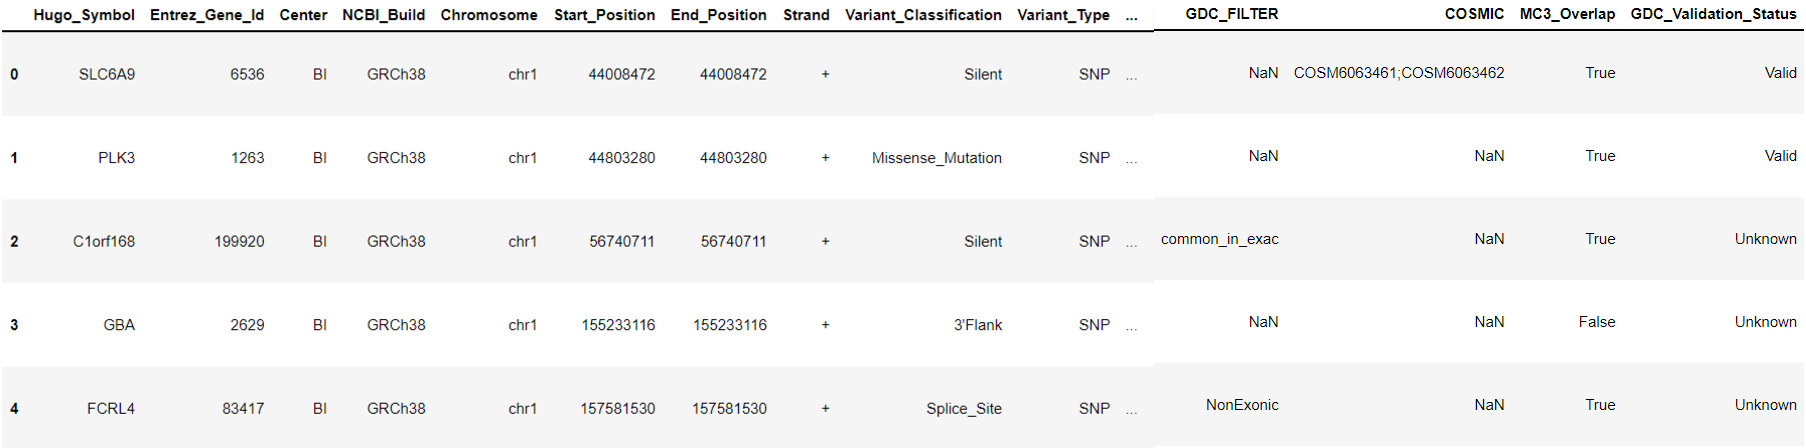
\includegraphics[width=0.99\textwidth,height=0.2\textheight]{Chapters/Figures/dataset.jpg}
    \caption{data set example}
    \label{fig:dataset}
\end{figure}

First and foremost, it is necessary to extract the independent variables and the dependent variables. Independent variables are all variables that are changed or controlled during a scientific experiment in order to test the effects on the dependent variables, so for our data set the independent variables will be "Hugo\_Symbol"\ and "Entrez\_Gene\_Id ", as they represent the identification of each mutation. On the other hand, the dependent variables are those that are tested and measured during the scientific experiment, that is, they will be the remaining columns of the data set, aka features. The code below shows the steps necessary to extract the two types of variables, Y being the independent variable and X the dependent variables. The focus will be on the variable "Entrez\_Gene\_Id"\ as the sole independent variable, being an integer variable it is easier and less laborious to preprocess it before applying the algorithms, "Hugo\_Symbol"\ will only be used for future validation if necessary.

\begin{lstlisting}[language=Python]
#independent variables 
    Hugo_Symbol = table.loc[:,["Hugo_Symbol"]]
    Y = table.loc[:,["Entrez_Gene_Id"]]
\end{lstlisting}
%%%
%%\begin{figure}[h]
   % \centering
    %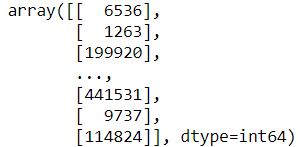
\includegraphics[width=0.4\textwidth,height=0.14\textheight]{Chapters/Figures/Y_var.png}
    %\caption{Y values}
    %\label{fig:Y_var}
%%\end{figure}

\begin{lstlisting}[language=Python]
#dependent variables
    X = table.drop(["Hugo_Symbol","Entrez_Gene_Id"], axis = 1)
\end{lstlisting}
%%%\begin{figure}[h]
    %\centering
    %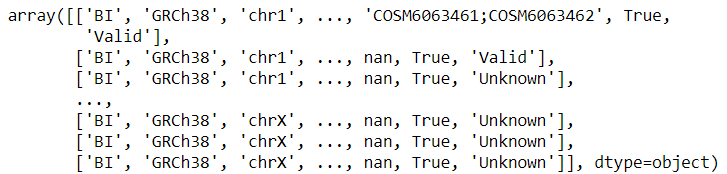
\includegraphics[width=0.95\textwidth,height=0.15\textheight]{Chapters/Figures/X_var.png}
    %\caption{X values}
    %\label{fig:X_var}
%%%\end{figure}
